\chapter{Movement}\label{ch:move}
For our robot to be able to show the results of path finding,
it needed to be able to move.

We decided to move only along a simple 2D grid-like structure,
therefore wheels were the easiest solution.
\todo{we need to make this flow nicer into the next section}

\section{Motors}\label{sec:motors}
A stepper motor is a motor that moves one step at a time, with its step defined by a step angle.

\begin{figure}[ht]
	\centering
	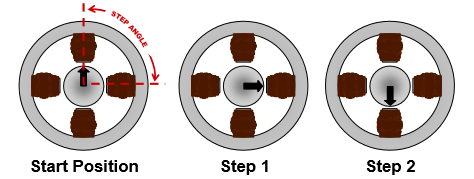
\includegraphics[width=\textwidth]{figures/move/motor1.png}
	\caption{Step Angle}
	\label{fig:angle} 
\end{figure}

Figure \ref{fig:angle} represents a stepper motor that requires 4 steps to complete a 360 degrees rotation. This determines the step angle to be 90 degrees.
The main components of a stepper motor are represented in Figure \ref{fig:main_components}, and they consist of stators, windings(phases), and rotor.
The part that moves, is the rotor, which can be magnetized or not, depending on the type of stepper motor.

\begin{figure}[ht]
	\centering
	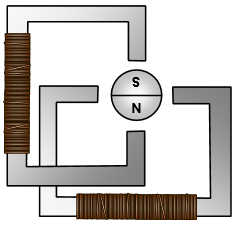
\includegraphics[width=0.5\textwidth]{figures/move/motor2.png}
	\caption{Main Components}
	\label{fig:main_components}
\end{figure}

By applying a voltage across one of the windings, current will start flowing through it. By using the right-hand rule, the direction of the magnetic flux can be determined. The flux will want to travel through the path that has the least resistance. This determines the rotor to change its position to minimize resistance. This is shown in Figure \ref{fig:flux}.

\begin{figure}[htp]
	\centering
	\subfloat[High Resistance]{%
		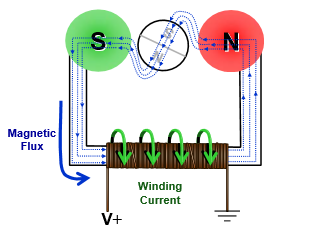
\includegraphics[width=0.4\textwidth]{figures/move/motor3.png}%
		}%
	\hfill
	\subfloat[Low Resistance]{%
		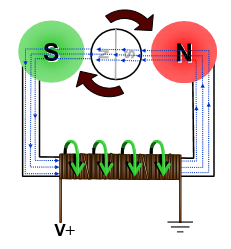
\includegraphics[width=0.4\textwidth]{figures/move/motor4.png}
	}
	\caption{Direction of Magnetic Flux}
	\label{fig:flux}
\end{figure}

\subsection{Types of Stepper Motors}
\subsubsection{Permanent Magnet Motor}
This type of stepper motor has a magnetized rotor. Each winding, will be subdivided into two, to better understand how to motor functions. Figure \ref{fig:bas_struct} represents the windings, and how they are distributed inside a stepper motor.

\begin{figure}[htp]
    \centering
    \subfloat[Rotor]{%
        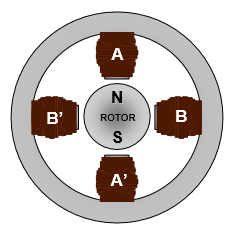
\includegraphics[width=0.4\textwidth]{figures/move/motor5.png}%
        }%
    \hfill%
    \subfloat[Winding]{%
        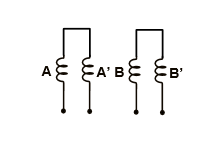
\includegraphics[width=0.4\textwidth]{figures/move/motor6.png}%
        }%
    \caption{Basic Structure of a Motor}
    \label{fig:bas_struct} 
\end{figure}

The resolution of the motor can be improved in two ways, either by increasing the number of pole pairs in the rotor itself, or by increasing the number of phases as shown in Figure \ref{fig:inc_res}.


\begin{figure}[htp]
    \centering
    \subfloat[Increased Pole Pairs]{%
        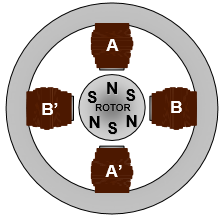
\includegraphics[width=0.4\textwidth]{figures/move/motor7.png}%
        }%
    \hfill%
    \subfloat[Increased Number of Winding]{%
        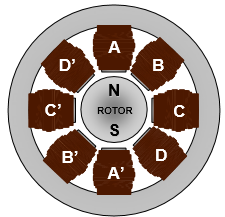
\includegraphics[width=0.4\textwidth]{figures/move/motor8.png}%
        }%
	\hfill%
	\caption{Increased resolution}
	\label{fig:inc_res}
\end{figure}

\newpage
To rotate the motor, simply apply a voltage across the windings in a sequence. A full rotation is shown in Figure \ref{fig:stepping_perm_magn}, with the corresponding phase energized.

\begin{figure}[htp]
    \begin{center}
    \subfloat[$1\textsuperscript{st}$ Step]{
        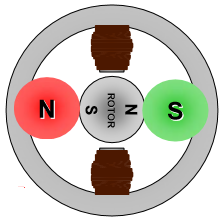
\includegraphics[width=0.2\textwidth]{figures/move/motor9.png}
        }
    \hfill
    \subfloat[$2\textsuperscript{nd}$ Step]{
        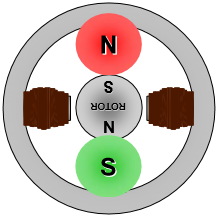
\includegraphics[width=0.2\textwidth]{figures/move/motor10.png}
        }
    \hfill
    \subfloat[$3\textsuperscript{rd}$ Step]{
    	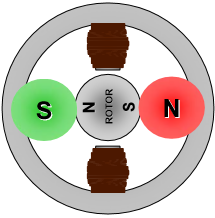
\includegraphics[width=0.2\textwidth]{figures/move/motor11.png}
    	}
  	\hfill
  	\subfloat[$4\textsuperscript{th}$ Step]{
  		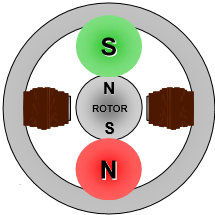
\includegraphics[width=0.2\textwidth]{figures/move/motor12.png}
  		}
    \end{center}
    
    \begin{center}
    \subfloat[$1\textsuperscript{st}$ Step Winding]{
        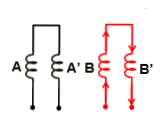
\includegraphics[width=0.2\textwidth]{figures/move/motor13.png}
        }
    \hfill
    \subfloat[$2\textsuperscript{nd}$ Step Winding]{
        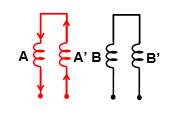
\includegraphics[width=0.2\textwidth]{figures/move/motor14.png}
        }
    \hfill
    \subfloat[$3\textsuperscript{rd}$ Step Winding]{
    	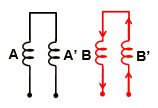
\includegraphics[width=0.2\textwidth]{figures/move/motor15.png}
    	}
  	\hfill
  	\subfloat[$4\textsuperscript{th}$ Winding]{
  		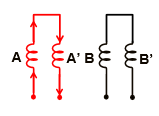
\includegraphics[width=0.2\textwidth]{figures/move/motor16.png}
  		}
  	\caption{Stepping a Permanent Magnet Motor}
  	\label{fig:stepping_perm_magn}
    \end{center}
\end{figure}

\subsubsection{Variable Reluctance Motor}
This type of motor, uses a rotor that is not magnetized, and has a number of teeth as seen in Figure \ref{fig:var_rel_components}. The windings are configured differently, as depicted in the second figure, all having a common voltage source but with each end being separate. They usually have 3 or 5 windings. Greater precision can be achieved by adding more teeth to the rotor.

\begin{figure}[htp]
    \centering%
    \subfloat[Non Magnetized Rotor]{%
        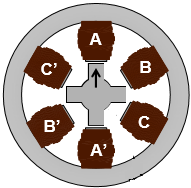
\includegraphics[width=0.3\textwidth]{figures/move/motor17.png}%
        }%
    \hfill%
    \subfloat[Windings]{%
        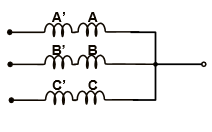
\includegraphics[width=0.4\textwidth]{figures/move/motor18.png}%
        }%
    \caption{Variable Reluctance Motor Components}%
    \label{fig:var_rel_components}%
\end{figure}
\newpage

To spin the motor, each winding is energized one at a time, and the rotor rotates in such a way, to minimize reluctance. Some of the differences, between this type of stepper motor and the permanent magnet motor, are that, in order to spin the motor in a direction, the windings have to be energized in a reverse sequence, as depicted in Figure \ref{fig:stepping_var_rel}. In addition, the step angle is actually half of the one of a permanent magnet motor with the same number of windings is.

\begin{figure}[htp]
    \begin{center}
    \subfloat[$1\textsuperscript{st}$ Step]{
        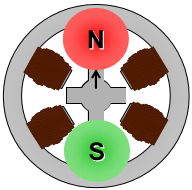
\includegraphics[width=0.2\textwidth]{figures/move/motor19.png}
        }
    \hfill
    \subfloat[$2\textsuperscript{nd}$ Step]{
        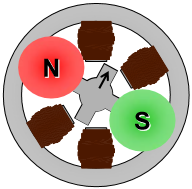
\includegraphics[width=0.2\textwidth]{figures/move/motor20.png}
        }
    \hfill
    \subfloat[$3\textsuperscript{rd}$ Step]{
    	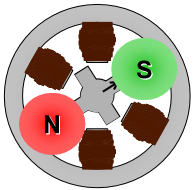
\includegraphics[width=0.2\textwidth]{figures/move/motor21.png}
    	}
  	\hfill
  	\subfloat[$4\textsuperscript{th}$ Step]{
  		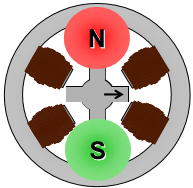
\includegraphics[width=0.2\textwidth]{figures/move/motor22.png}
  		}
	\end{center}
	\begin{center}
    \subfloat[$1\textsuperscript{st}$ Step Winding]{
        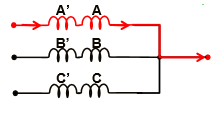
\includegraphics[width=0.2\textwidth]{figures/move/motor23.png}
        }
    \hfill
    \subfloat[$2\textsuperscript{nd}$ Step Winding]{
        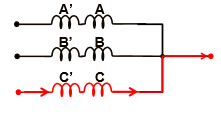
\includegraphics[width=0.2\textwidth]{figures/move/motor24.png}
        }
    \hfill
    \subfloat[$3\textsuperscript{rd}$ Step Winding]{
    	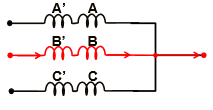
\includegraphics[width=0.2\textwidth]{figures/move/motor25.png}
    	}
  	\hfill
  	\subfloat[$4\textsuperscript{th}$ Winding]{
  		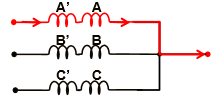
\includegraphics[width=0.2\textwidth]{figures/move/motor26.png}
  		}
  	\caption{Stepping Variable Reluctance Motor}
  	\label{fig:stepping_var_rel}
  	\end{center}
\end{figure}
\newpage
\subsubsection{Hybrid Stepper Motor}
Hybrid stepper motors borrow characteristics both the previous ones. Figure \ref{fig:hybrid_components} shows the two of the main components of the hybrid stepper motor. On the left side, the stator can be seen consisting of 8 poles. On the right side, is represented the rotor. The rotor consists of two sets of teeth, corresponding for the two poles, north and south, respectively.

\begin{figure}[h]
	\centering
	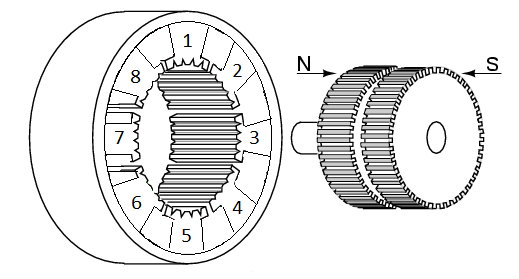
\includegraphics[width=\textwidth]{figures/move/motor27.png}
	\caption{Stator And Rotor}
	\label{fig:hybrid_components}
\end{figure}

It is important to notice two additional things. The first, is that the teeth on the rotor are not aligned but are interleaved. The second, is the placement of the stator teeth in respect to those of the rotor. Both can be observed in Figure \ref{fig:stepper}.

\begin{figure}[htp]
    \centering%
    \subfloat[Interleaved Teeth]{%
        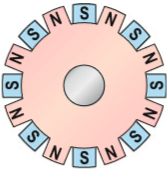
\includegraphics[width=0.4\textwidth]{figures/move/motor28.png}%
        }%
    \hfill%
    \subfloat[Stepper Motor Inside]{%
        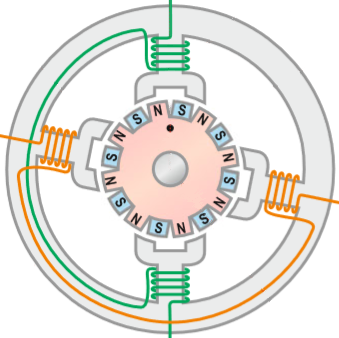
\includegraphics[width=0.3\textwidth]{figures/move/motor29.png}%
        }%
    \caption{Hybrid Stepper Motor}
    \label{fig:stepper}
\end{figure}
\newpage
Figure \ref{fig:stepper}, the windings with numbers 1 and 5 are completely aligned with the teeth of the rotor. Windings number 3 and 7 are completely unaligned, while the others are half aligned. This results in higher precision and higher torque offered by the hybrid stepper motor, depending on the stepping method used.

Figure \ref{fig:hybrid_stepper} the front view of the hybrid stepper motor together with the configuration of the two windings.

\begin{figure}[htp]
    \centering%
    \subfloat[Front View Stepper Motor]{%
        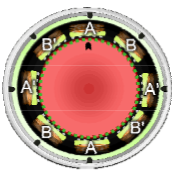
\includegraphics[width=0.4\textwidth]{figures/move/motor30.png}%
        }
    \hfill%
    \subfloat[Winding Configuration]{%
        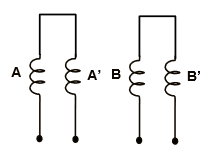
\includegraphics[width=0.4\textwidth]{figures/move/motor31.png}%
        }%
    \caption{Hybrid Stepper Motor Configuration}%
    \label{fig:hybrid_stepper}
\end{figure}

It is important to notice that, even though the motor has only two windings, each individual winding energizes 4 stator poles.

Figures \ref{fig:hybrid_first_step},  \ref{fig:hybrid_second_step}, \ref{fig:hybrid_third_step} represent the way this motor operates.

\begin{center}
	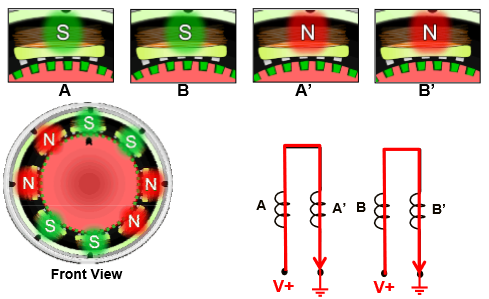
\includegraphics[width=0.8\textwidth]{figures/move/motor32}
	\captionof{figure}{First Step}
	\label{fig:hybrid_first_step}
\end{center}
\newpage
By applying a voltage to both windings, the current flow can be controlled, thereby controlling the polarity of each stator pole, thus controlling the direction of the motor. Notice that, initially, poles A and A’ are completely aligned, and poles B and B’ are half aligned. 

\begin{center}
	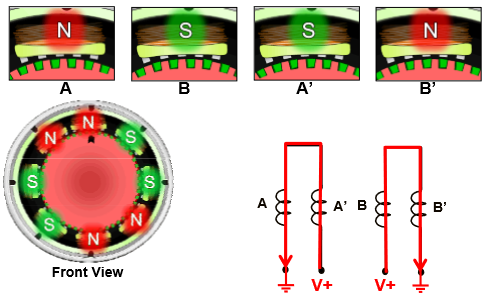
\includegraphics[width=0.8\textwidth]{figures/move/motor33}
	\captionof{figure}{Second Step}
	\label{fig:hybrid_second_step}
\end{center}

Next step involves changing the direction of the current in winding A by applying a voltage at the other end of the winding. Even though only the current in winding A has been changed, all stator poles are aligned differently. Poles A and A’ are now half aligned, and poles B and B’ are completely aligned.

\begin{center}
	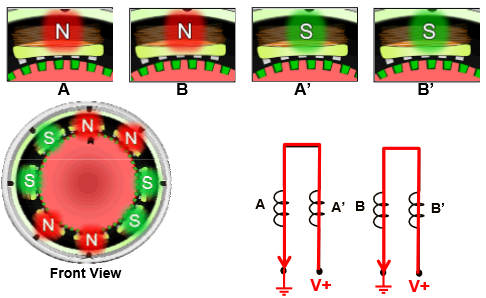
\includegraphics[width=0.8\textwidth]{figures/move/motor34}
	\captionof{figure}{Third Step}
	\label{fig:hybrid_third_step}
\end{center}
\newpage
Now, changing the direction of the current in winding B, changes the polarity of the stator poles B and B', again, determining a change in the alignment of all stator poles. A and A’ are now completely aligned, and stator poles B and B’ are half aligned. The positions of the stator poles now correspond to those of the first step.

\begin{center}
	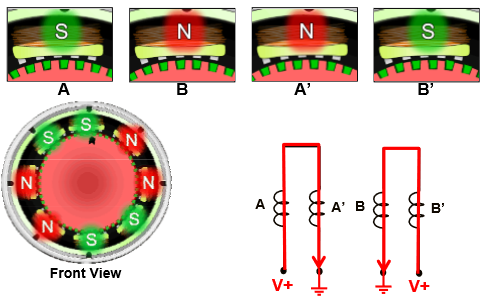
\includegraphics[width=0.8\textwidth]{figures/move/motor35}
	\captionof{figure}{Forth Step}
	\label{fig:hybrid_forth_step}
\end{center}


Finally, again changing the direction of the current in winding A, determines the rotor to move another step. Notice the alignment of the stator poles. A and A’ are half aligned, while B and B’ are fully aligned. By changing the direction of the current in winding B, the motor arrives in the initial state, thus repeating the sequence.
\newpage

\subsection{Unipolar And Bipolar Stepper Motors}

Another classification of stepper motors, is depending on the way the windings are configurated. Even though, nowadays, almost every stepper is both. Meaning that unipolar and bipolar, are rather modes in which the stepper motor can be driven. Exception being, stepper motors which have only four wires coming out of them, corresponding to bipolar stepper motors.

Figure \ref{fig:windings} below represent the configuration of the windings in both unipolar and bipolar stepper motors. 


\begin{figure}[htp] 
    \centering
    \subfloat[Bipolar]{
        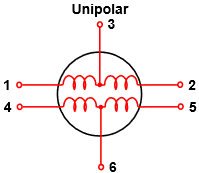
\includegraphics[width=0.4\textwidth]{figures/move/motor36.png}
        }
    \hfill
    \subfloat[Unipolar]{%
        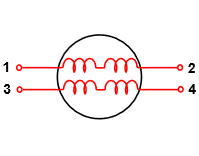
\includegraphics[width=0.4\textwidth]{figures/move/motor37.png}
        }
    \caption{Winding Configuration}
    \label{fig:windings}
\end{figure}

Unipolar stepper motors allow current flow in only one direction through the winding, so a center wire has been added, that provides a voltage and determines the stator poles to either be of north or south polarity. Unipolar stepper motors are widely used in applications that require high torque at high speed.

Bipolar stepper motors, allow current to flow in both directions through the windings, so the need of a center wire to provide a voltage disappears. However, the circuit needed to drive a bipolar stepper motor is more complicated. Bipolar stepper motors driving boards exist to make it easier for a person to program the motor. Bipolar stepper motors are used in applications that require high torque at low speeds.
\newpage
Figure \ref{fig:unipolar_stepping} better explains the operating method of unipolar stepper motors. 

\begin{figure}[htp] 
    \centering
    \subfloat[$1\textsuperscript{st}$ Step]{
        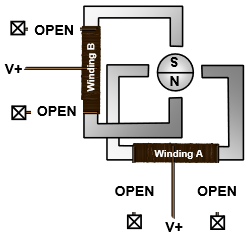
\includegraphics[width=0.3\textwidth]{figures/move/motor38.png}
        }
    \hfill
    \subfloat[$2\textsuperscript{nd}$ Step]{
        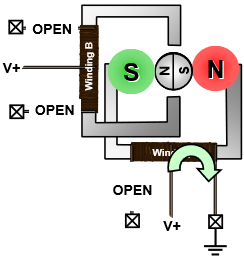
\includegraphics[width=0.3\textwidth]{figures/move/motor39.png}
        }
    \hfill
    \subfloat[$3\textsuperscript{rd}$ Step]{
    	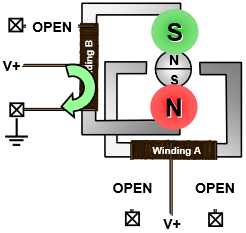
\includegraphics[width=0.3\textwidth]{figures/move/motor40.png}
    	}
  	\hfill
  	\subfloat[$4\textsuperscript{th}$ Step]{
  		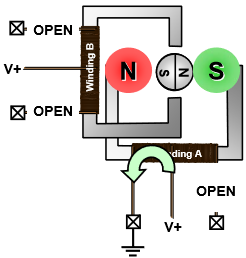
\includegraphics[width=0.3\textwidth]{figures/move/motor41.png}
  		}
  	\hfill
  	\subfloat[$5\textsuperscript{th}$ Step]{
  		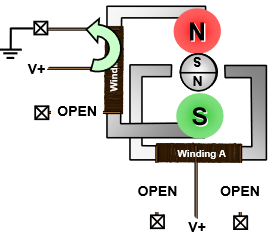
\includegraphics[width=0.3\textwidth]{figures/move/motor42.png}
  		}
  	\caption{Unipolar Motor Stepping}
  	\label{fig:unipolar_stepping}
\end{figure}

As seen in Figure \ref{fig:unipolar_stepping}, each step only uses half of the winding, determining the polarity of the stator poles. The voltage is always applied at the same wire two wires.
\newpage
Note that the bipolar configuration as shown in Figure \ref{fig:bipolar_stepping} allows the current to flow in both directions, but the voltage and ground continuously switch positions. This makes bipolar stepper motors a bit more complicated to drive, but as previously stated, motor driver boards simplify the task.

\begin{figure}[htp] 
    \centering
    \subfloat[$1\textsuperscript{st}$ Step]{
        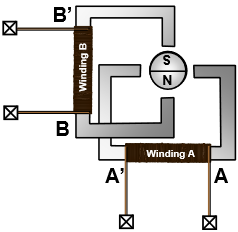
\includegraphics[width=0.3\textwidth]{figures/move/motor43.png}
        }
    \hfill
    \subfloat[$2\textsuperscript{nd}$ Step]{
        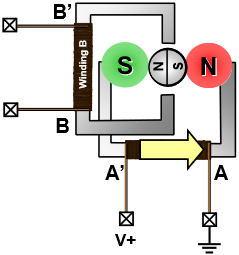
\includegraphics[width=0.3\textwidth]{figures/move/motor44.png}
        }
    \hfill
    \subfloat[$3\textsuperscript{rd}$ Step]{
    	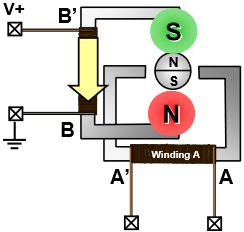
\includegraphics[width=0.3\textwidth]{figures/move/motor45.png}
    	}
   	\hfill
   	\subfloat[$4\textsuperscript{th}$ Step]{
  		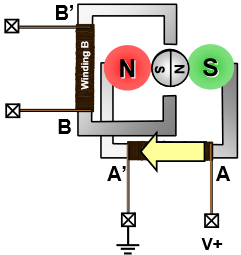
\includegraphics[width=0.3\textwidth]{figures/move/motor46.png}
  		}
  	\hfill
  	\subfloat[$5\textsuperscript{th}$ Step]{
  		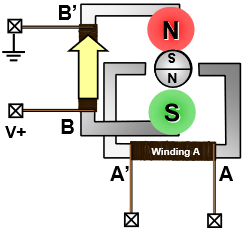
\includegraphics[width=0.3\textwidth]{figures/move/motor47.png}
  		}
  	\caption{Bipolar Motor Spinning}
  	\label{fig:bipolar_stepping}
\end{figure}
%\section{Tri-State Buffer}\label{sec:buffer}
\newpage
\section{Wheels}\label{sec:wheels}
The robot should be able to move in eight directions from every position. By using traditional wheels, the robot should be able to steer to the desired direction, thus changing orientation. This would have been a difficult task rising a number of problems. Our solution is to use omni-wheels instead. A standard wheel and an omni-wheel are shown in Figure \ref{fig:wheels}.

Omni-wheels look like traditional wheels, but their contact area consists of smaller wheels that are able to move freely. By mounting the wheels in pairs, with the shafts crossing at a 90$^\circ$ angle, we are able to move the robot in any of the eight direction without needing to change the orientation of the robot.

\begin{figure}[htp]
	\centering
	\subfloat[Standard Wheel]{
		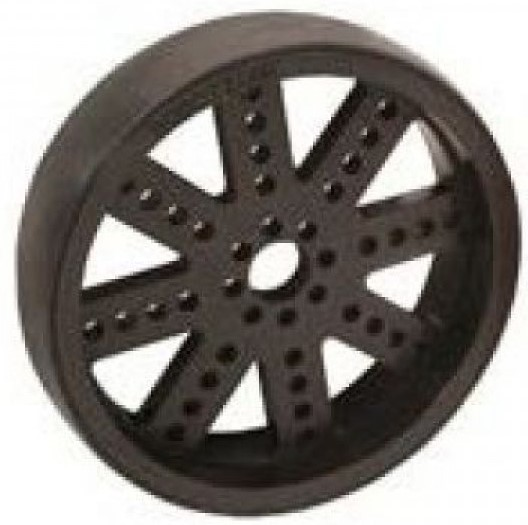
\includegraphics[width=0.26\textwidth]{figures/move/regular_wheel}
	}
	\hfill
	\subfloat[Omni-Wheel]{
		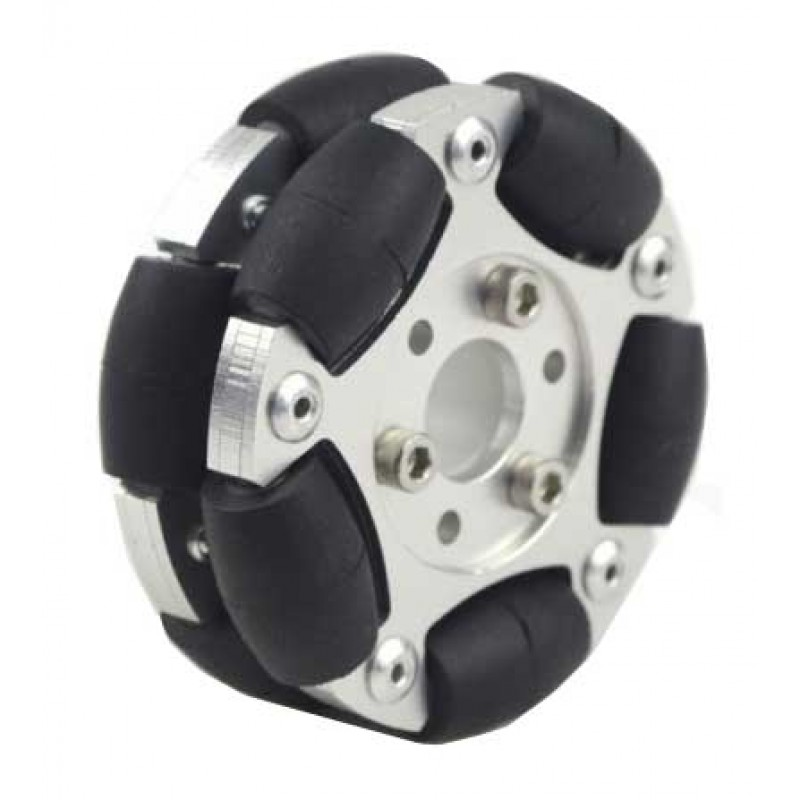
\includegraphics[width=0.26\textwidth]{figures/move/omni_wheel}
	}
	\caption{Wheels}
	\label{fig:wheels}
\end{figure}
\begin{figure}[htp]
	\begin{center}
    \subfloat[North]{
    	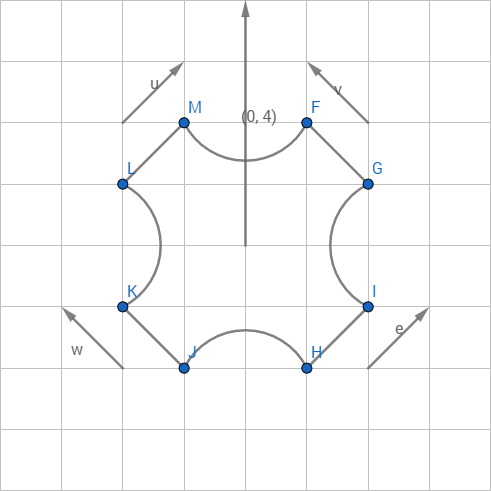
\includegraphics[width=0.3\textwidth]{figures/move/vector_addition_North}
    }
    \subfloat[West]{
    	\includegraphics[width=0.3\textwidth]{figures/move/vector_addition_East}
    }
    \end{center}
    \begin{center}
    \subfloat[South]{
   		\includegraphics[width=0.3\textwidth]{figures/move/vector_addition_South}
    }
  	\subfloat[East]{
 		\includegraphics[width=0.3\textwidth]{figures/move/vector_addition_West}
	}
	\end{center}
	\begin{center}
    \subfloat[North-East]{
    	\includegraphics[width=0.3\textwidth]{figures/move/wheel_vectors_NE}
    }
    \subfloat[South-East]{
   		\includegraphics[width=0.3\textwidth]{figures/move/wheel_vectors_SE}
    }
    \end{center}
    \begin{center}
    \subfloat[South-West]{
    	\includegraphics[width=0.3\textwidth]{figures/move/wheel_vectors_SW}
    }
  	\subfloat[North-West]{
  		\includegraphics[width=0.3\textwidth]{figures/move/wheel_vectors_NW}
	}
	\end{center}
  	\caption{Forces from Multiple Wheels Added Together}
  	\label{fig:forces}
\end{figure}
Figure \ref{fig:forces} shows in which direction each motor has to spin in order for the robot to move in one of the eight directions. It can also be observed that no two opposite motors spin in different directions. This has also made our task of programming the motors easier. 
\clearpage
\section{Tri-State Buffer}
\clearpage
\section{Motor Drive Boards}\label{sec:driver_boards}
\clearpage
\section{Direction Control}\label{sec:direction}
To determine the direction of the robot, we had to determine which wheels turn what number of steps. 

One option would have been to control each motor individually. This required a significant number of pins needed for stepping the motors, and precise timing between the four motors, considering that, in some instances all motors should move at the same time.

We decided to use tri-state buffers instead. This would drastically lower the number of pins needed, and would make for a more precise and advanced way of driving the motors.

Table \ref{table:directions} explains which pairs need to be activated or not, and their rotation, in order to achieve the desired movement.

\begin{center}
	\begin{tabular}{|l|l|l|}
		\hline
		Direction & Pair A & Pair B	\\
		\hline
		North & forward & forward \\
		East 	& forward & backward \\
		South & backward & backward \\
		West 	& backward & forward \\
		\hline
		North-East & forward & off \\
		South-East & off & backward \\
		South-West & backward & off\\
		North-West & off & forward \\
		\hline
	\end{tabular}
	\begin{tabular}{|l|c|c|c|c|}
		\hline
		Direction & Aon & Aflip & Bon & Bflip \\
		\hline
		North & 1 & 0 & 1 & 0 \\
		East 	& 1 & 0 & 1 & 1 \\
		South & 1 & 1 & 1 & 1 \\
		West 	& 1 & 1 & 1 & 0 \\
		\hline
		North-East & 1 & 0 & 0 & 1 \\
		South-East & 0 & 1 & 1 & 0 \\
		South-West & 1 & 1 & 0 & 1 \\
		North-West & 0 & 1 & 1 & 1 \\
		\hline
	\end{tabular}
	\captionof{table}{Directions}
	\label{table:directions}
\end{center}



\begin{figure}[htp]
	\centering
	\includegraphics[width=0.9\textwidth]{figures/move/direction_choice}
	\caption{Motor Control Circuit}
	\label{fig:mot_ctrl}
\end{figure}

We decided to use 6 tri-state buffers as shown in figure \ref{fig:mot_ctrl}.
